

\documentclass[12pt]{article}
\usepackage[T1]{fontenc}
\usepackage[utf8]{inputenc}
\usepackage{amsmath}
\usepackage{microtype}
\usepackage{listings}
\setlength{\parindent}{0pt}
\usepackage{fancyvrb}
\usepackage{enumerate}
\usepackage{array}
\usepackage[breaklinks=true,linktocpage,hidelinks]{hyperref}
\usepackage[letterpaper]{geometry}
\usepackage{url}
\usepackage{graphicx}
\usepackage{fullpage}

\usepackage{pgfplots}
\usepackage{pgfplotstable}
\usepackage{tikz}

\usepackage{fancyhdr}
\usepackage{fancybox}
\usepackage{multicol}
\usepackage{xcolor}
\usepackage{adjustbox}

\pgfplotsset{compat=newest}
\usetikzlibrary{shapes,backgrounds,arrows}
\usepgfplotslibrary{external} 

\definecolor{brewcol1}{RGB}{166,206,227}
\definecolor{brewcol2}{RGB}{31,120,180}
\definecolor{brewcol3}{RGB}{178,223,138}
\definecolor{brewcol4}{RGB}{51,160,44}
\definecolor{brewcol5}{RGB}{251,154,153}
\definecolor{brewcol6}{RGB}{227,26,28}
\definecolor{brewcol7}{RGB}{237,179,1}
\definecolor{brewcol8}{RGB}{202,178,214}
\definecolor{brewcol9}{RGB}{206,27,1}

\geometry{hmargin=1.87cm, vmargin=1.87cm}
\bibliographystyle{siam}

\DeclareTextFontCommand{\helvetica}{\fontfamily{phv}\selectfont\small}


\begin{document}

\clearpage\thispagestyle{empty}
\begin{center}
\textbf{Difficult transition for sugar maple in Boreal forest under climate change? \\
Impact of alternative stable states on Sugar maple migration.}
\vskip 2em
Research proposal
\vskip 1em
Master in Wildlife management
\vfill
By
\vfill
Steve Vissault 
\vfill 
For
\vfill
\textbf{Richard Cloutier}, Pr.\\
Director of the program committee
\vskip 2em
\textbf{Dominique Arsenault}, Pr.\\
President of the jury
\vskip 2em
\textbf{Matt Talluto}, PhD\\
Research Co-director
\vskip 2em
\textbf{Dominique Gravel}, Pr.\\
Research Director
\vfill
\vfill
Université du Québec à Rimouski\\
\today

\end{center}

\newpage
\setcounter{page}{1}

\section{Introduction}

\textbf{Context.}  The boreal region is warming twice as fast as the global
average and  this will inevitably alter the species composition in boreal
forests \cite{Scheffer2012,Hughes2000,Lafleur2010}. Sugar maple (\textit{Acer
saccharum}) is a widespread and abundant tree in north-eastern North America.
\cite{Graignic2013,Messaoud2007,Kellman2004,Barras1998}. Predicting shifts in
the range of Sugar maple is an important challenge because this species is
highly desirable by hardwood and maple syrup producers, two large economic
sectors in Quebec. Some species mostly representative of northern forest
ecosystems are forecast to expand their distribution broadly towards the north
\cite{Sciences2014,Iverson2002}. According to McKenney (20007), Sugar maple is
one of those species expected to move closed to the Ungava bay
\cite{Sciences2014}. This species is dominating the northern temperate forest
especially along the boreal-temperate forests ecotone at its northern range
limit \cite{Barras1998}. Actually, Sugar maple predictions are built on
species distribution models based only on climatic conditions, though Sugar
maple regeneration depends both on macro conditions (\textit{i.e.} regional
climate) and micro conditions (\textit{i.e.} soil and microtopography)
\cite{Graignic2013,Lafleur2010}. Thus, the expansion of Sugar maple and his
temperate species community is difficult to predict because micro conditions
can mitigate macro conditions such as global warming \cite{DeFrenne2013}.\\

Species are responding differently to the soil conditions, and the soil
properties found in boreal forests are different from those in temperate
forest \cite{Lafleur2010,Barras1998,Goldblum2010,Demers1998}. Conifer forests
generally contain deep and poorly-decomposed litter to layers, while those of
northern hardwood forests are thinner but covered by a tough superficial leaf
mat \cite{Barras1998}. In boreal forest, the temperature is colder and the
snow melts later, the soil is wetter and the litter is more acidic and fibrous
\cite{Lafleur2010,Goldblum2010}. Soil acidification is causing a reduction in
the cation exchange capacity and subsequently decrease avaibility of some
nutrients such as calcium \cite{Moore2008}. Sugar maple regeneration has been
recognized to be particulary sensitive to waterlogged condition and nutrients
soil content \cite{Moore2008,Lafleur2010,Cleavitt2011}. This properties of
coniferous forest soils could hinder the local establishment of species
associated with base-rich soils or unable to withstand waterlogged conditions
\cite{Lafleur2010}. Under these latter conditions, tree species migration is
likely to be restricted or delayed \cite{Lafleur2010}. Thus even if the
regional climate conditions are favorable, the micro conditions found in the
boreal forest could slowing down the seedling establishment of these temperate
species \cite{Kellman2004,Moore2008,Barras1998,Messier2011}. Then the
temperate forest including Sugar maple could then be unable to migrate in
boreal forests as a result of local plant-soil feedbacks
\cite{McCarthyNeumann2012}. To study the expansion of Sugar maple, the ecotone
dynamic can be conceptualized through two set of dominant species communities:
the boreal community and the temperate community including Sugar maple. The
landscape might be structured as a patchy mosaic structure where micro
conditions are driving the spatial occurences of boreal and temperate
community species despite a regional climate favorable to temperate species
\cite{Goldblum2010,Fisichelli2013}. In this case, these forest communities are
two alternative stable states, \textit{i.e.} contrasted states occuring in the
same climate conditions \cite{scheffer2009critical}. This situation generate a
tension between the boreal and temperate forest meaning that modification on
micro conditions (i.e mainly soil conditions) can produce abrupt shift in
community composition in the boreal-temperate forest ecotone.\\

\textbf{Objectives.} The main objective of this project is to investigate the
transition between the boreal and temperate forests under different climate
change scenarios. In this context, we will test two different hypothesis:
($H_1$) Alternative stable states are occuring in the boreal-temperate forests
ecotone;  ($H_2$) Time lags in the response to climate change will be larger
in areas where alternative stable states are occuring. In order to achieve my
general objective and test these hypotheses, we will (1) develop a climate-
dependent model of state transition (STM) representing the dynamics of the
boreal and temperate communities at landscape scale; (2) investigate the
spatial structure of maple distribution through his temperate community; (3)
Study the occurrence of alternative stable states in the transitional zone;
and finally (4) run simulations of the temperate community species
distribution under different climate change scenarios. The first section of
this proposal reviews the context of the study. The first part of the review
presents the concept of alternative stable states and critical transitions in
forest ecosystem properties. The second part focuses on Sugar maple, it's
associated community in the temperate biome and a justification about why
alternative stable states are expected to occure at the boreal-temperate
forests ecotone. The last section of this document describes the model and
the methodology that we will employ to fill my specific objectives. 

\section{Review} 

\begin{figure}[t]
	\begin{center}
	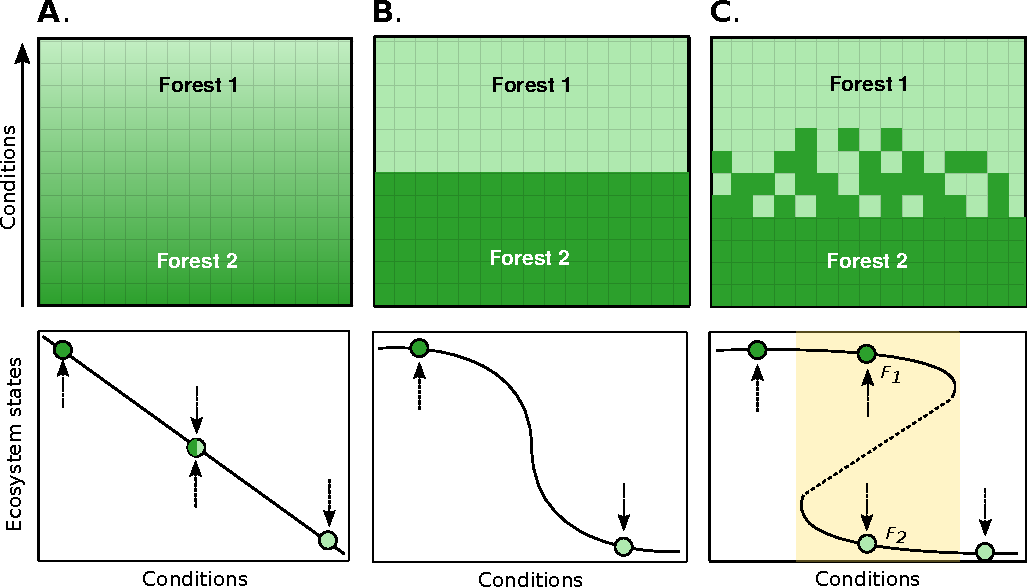
\includegraphics[width=0.8\textwidth]{fig/states.pdf}
	\end{center}
	\caption{Schematic representation of different ways in which the equilibrium
	states from forest-forest system can vary over environnemental gradients such as temperature, precipitation
	or soil moisture. Three differents responses are presented,
	\textbf{(A)} gradual, \textbf{(B)} basic fold, \textbf{(C}) catastrophic fold.
	The first line presents the stable states rise by the forest
	given a specific environnemental condition. Arrows indicate the
	direction the system moves if not at the equilibrium. 
	Solid lines represent stable states along the boreal-temperate
	transition, and the dashed line (in yellow highlight) unstable equilibrium. This zone,
	called hysteresis, is particulary unstable and small fluctuations in
	environnement conditions give rise to a contrasted state representing an
	alternative stable states. ($F_1$ or $F_2$). 
	The second line illustrates a conceptualization of a transitional landscape
	between the boreal (light green) and the nordic temperate forests (dark
	green).}
	\label{fig1}
	\vspace{-1.25em}
\end{figure}


\textbf{Alternative stable states in forest ecosystems.} The idea that
alternative stable states may exist in community ecology has been emerged
since the late 1960s \cite{Scheffer2001,Society2014a}. May (1977) highlights
the fact than a ecosystem can be seen as a dynamic system where species
communities possess several different equilibrium points named alternative
stable states \cite{May1977}. Suppose that a forest ecosystem can be usefully
characterized by a set of dynamic state variables, with their relations to
each other defined by a set of climate conditions. In the present context, a
state is defined as a forest species community given a time and a set of
climate conditions (e.g. annual precipitation and annual temperature). Changes
on this set of parameters can induce three different shapes of ecosystem
response \textbf{(A)} gradual, \textbf{(B)} basic fold, \textbf{(C})
catastrophic fold  \cite{Scheffer2001} (Figure \ref{fig1}, upper panel).
Firstly, when a small environmental change occur forest ecosystems can respond
almost linearly, with no threshold leading to drastic changes in the species
community (Figure \ref{fig1}.a, upper line) \cite{Scheffer2001,Scheffer2009}.
In this case, forest ecosystems can be seen rather as a continuum of states
along the climate gradient
\cite{Scheffer2001,Scheffer2009,scheffer2009critical}. For instance, when the
annual precipitation increase slightly in a forest deciduous stand, the new
local condition gives rise to a new coniferious species establishment (e.g
balsam fir). This forest stand reaches a new state wherein the species
community has been smoothly changed. Secondly, such forest ecosystems are
insensitive to small change in environmental conditions over certain ranges
but respond strongly when a threshold is reached \cite{scheffer2009critical}.
For example, species mortality can increase sharply when the water level of a
lake is rising permanently in response to changing hydrologic conditions in
the drainage basin. The new condition change abruptly the entire species
assemblage surrounding the lake. Hence, the response curve of the natural
systeme is not linear but lightly folded and these change can drive the forest
ecosystem to a treshold and lead to major changes in the community (Figure
\ref{fig1} .b, upper line). Lastly, in some non-linear systems the response
curve can be folded backwards and alternative stable states could occur
(Figure \ref{fig1} .c).

% Facilitation et coller davantage à la dynamique forestière.

When the system approach a tipping point on the folded upper branch, it cannot
pass smootly to the lower branch. Small forcing on initial condition of the
state $F_1$ transfer immediatly the system into a contrasted state $F_2$
(Figure \ref{fig1} .c). This point is called a bifurcation point and a small
forcing on it can drive the system into backward or forward shifts.  In this
situation, the system present alternative stable states. Thus, over a range of
climate conditions, intermixed of constrasted patches can be observed in the
ecotone \ref{fig1} .c (lower line).\\

\textbf{Natural system studied.} Many empirical and modeling studies have been
conducted on the transition between forest to non- forests (e.g. Boreal-
Tundra) \cite{Scheffer2012,Scheffer2001,Hirota2011,Messaoud2007} but little
attention has been given to evaluate the forest-forest ecotone
\cite{Goldblum2010,Graignic2013,Messaoud2007}. At landscape scale, transition
between  the temperate and boreal forests can be approached as a dynamical
system where each forest biome community is a stable state. There is no
distinct boundary at the boreal-temperate ecotone instead a broad transition
zone exists where stands of coniferous deciduous species co-occur at the
regional scale \cite{Goldblum2010,Fisichelli2013}. A macromosaic landscape can
be observed with either pure stands of northern temperate trees or boreal
forest stands \cite{Goldblum2010,Fisichelli2013}. In this study context,
alternative stabe state theory could applied to the hardwood-boreal forest
patchiness structure often attribute to differences in soils, nutrient status
and topographical factors \cite{Society2014}. This segregated patches
distribution could be explain by the fact than microclimatic conditions can
modulate establishement of those forests \cite{DeFrenne2013}. Distribution of
deciduous and boreal forests within the ecotone is not determined by
macroclimatic conditions, but rather by local variation of substrate,
drainage, physical soil properties, and nutrient avaiblity
\cite{Goldblum2010,Society2014}.


%DG: strange wording, should'nt be the opposite, ie that specific conditions are associated (consequent) to tree composition?

Boreal and hardwood forests are dominated by trees with different physiognomy,
which is expected to produce distinctive litter and light micro-environments
\cite{Barras1998}.  A positive feedback contribute to the maintenance of the
community type if the dominant tree species promotes conditions facilitating
its own regeneration \cite{Barras1998}. Frelich \textit{et al.}(1993)
\cite{Society2014} hypothesized that Sugar maple is subject to such a
feedback.  Knowing this, the alternative stable states is a relevant framework
to study the ecotone dynamic. Soil conditions and role of dominant
species in regeneration seems to act as main feedbacks on the temperate forest
establishment generating a patchiness landscape (Figure \ref{fig1}.c, upper
panel).

%DG: reword the previous sentenc, unclear

In this context, we expected to find patch dominated by boreal species and
others dominated by temperate species under a certain range of climatic
conditions. Thus, the soil condition and the role of dominant species in
boreal and temperate forest need to be investigate as main drivers in
alternative stable states
\cite{Kellman2004,Moore2008,DeFrenne2013,Barras1998}.

%MT: Good summary. You might come back to climate change here, as well, to remind the reader that you will also be testing some hypotheses about climate change.
%DG: not clear what you mean at the previous sentence.

\section{Methods}   

\begin{wrapfigure}{L}{0.45\textwidth}
	
\begin{center}
	
				\tikzstyle{noeud}=[circle,
				                  thick,
				                  minimum size = 1.5cm,
				                  inner sep =5pt,
				                  draw=brewforest3,
				                  fill=brewforest1]
				\tikzstyle{noeud2}=[circle,
				                  thick,
				                  minimum size = 1.5cm,
				                  inner sep =5pt,
				                  draw=brewforest3,
				                  fill=brewforest3]
				\tikzstyle{noeud3}=[circle,
				                  thick,
				                  minimum size = 1.5cm,
				                  inner sep =5pt,
				                  draw=brewforest3,
				                  fill=brewforest3]
	
				\begin{tikzpicture}[->,>=stealth',auto,scale=0.65]
				      \node [circle,noeud2] (M) at (0,0) {\color{white}\textbf{M}};
				      \node [circle,noeud2]  (C) at (-5,5) {\color{white}\textbf{C}};
				      \node [circle,noeud2] (D) at (5,5) {\color{white}\textbf{D}};
				      \node [circle,noeud2] (T) at (0,10) {\color{white}\textbf{T}};
	
						\draw[thick,-latex] (M) to[bend right=10] node[above,sloped] {$S_C$} (C);
						\draw[thick,-latex] (C) to[bend right=10] node[below,sloped] {$\beta_d \cdot (D+M)$} (M);
	
						\draw[thick,-latex] (D) to[bend right=10] node[above,sloped] {$\beta_c \cdot (C+M)$} (M);
						\draw[thick,-latex] (M) to[bend right=10] node[below,sloped] {$S_D$} (D);
	
						\draw[thick,-latex] (D) to[bend right=10] node[above,sloped] {$e$} (T);
						\draw[thick,-latex] (T) to[bend right=10] node[below,sloped] {$\phi_D$} (D);
	
						\draw[thick,-latex] (T) to[bend right=10] node[above,sloped] {$\phi_C$} (C);
						\draw[thick,-latex] (C) to[bend right=10] node[below,sloped] {$e$} (T);
	
						\draw[thick,-latex,transform canvas={xshift=0.8ex}] (T) to node[above,sloped,rotate=90,transform canvas={xshift=3ex}] {$\phi_M $} (M);
						\draw[thick,-latex,transform canvas={xshift=-0.8ex}] (M) to node[above,sloped,rotate=-90,transform canvas={xshift=-3ex}] {$e$} (T);
				\end{tikzpicture}
	\end{center}	


	\caption{Conceptual representation of the transition model between deciduous ($D$),
	mixed ($M$) and coniferous ($C$) stands. $T$ corresponds to a post-disturbance forest patch. Perturbations, natural and anthropogenic, occur with a frequence $\epsilon$. Parameters $\theta$ and $\beta$ are rates of colonization and succession,
	respectively. We define recovery functions $\phi_c$ , $\phi_d$ as $\phi_c
	= \alpha_c \cdot (M+C) \cdot [1- \alpha_d \cdot (D+M)]$ and $\phi_d =
	\alpha_d \cdot (D+M) \cdot [1- \alpha_c \cdot (C+M)]$. $\phi_m$ include these both equations giving $\phi_m = \phi_c \cdot \phi_d$. Finally, parameter $\alpha$ represents the climate-dependent recovery rate after a patch has been disturbed.}
	\label{Model}
	\vspace{-1em}
\end{wrapfigure}


\textbf{State and Transitional Model.} The framework of this study lies on the
STM representing dynamics in the boreal-temperate forests transition at
landscape scale.  In overall, the ecotone landscape includes three distinctive
kind of forest canopies: (i) hardwood, (ii) mixedwood and finally (iii)
softwood \cite{Fisichelli2013}. Each of these stands are represented as a
state in the STM: \textbf{(D)} Deciduous, \textbf{(M)} Mixed and \textbf{(C)}
Coniferous (see green circle, figure \ref{Model}). According to Briske\textit{
et al.} (2008) and this STM context, state mean a plant community phases
occurring on similar soils that interact with the environment to produce
persistent functional and structural attributes. Flows or transition rates
between states are represented by arrows (figure \ref{Model}). Theses rates
are climate-depend. Transitions between all states are possible  except the
direct transition between a deciduous and coniferous stands, which does not
occur because it systematically require an intermediate step in state M.
Except for the colonisation rate ($\theta$), transition rates are varying with
the proportion of coniferious or deciduous available in the closest
neighbourhood. For instance, the succession rate of a coniferous patch
($\beta_c$) towards a mixed patch (M) depend also of the availability in C and
M patches in the landscape (figure \ref{Model}). Some disturbances might
change state proportion in the landscape. Natural disturbances is an important
driver of forest dynamics at landscape scale (e.g. fire in boreal forest or
large windthrow in temperate forest). For instance, small fires induce
deciduous dominance and larger and intense fires favoring boreal communities
\cite{Bergeron2004}. Anthropogenic disturbances such as logging can also
produce major change in the forest composition. Dupuis \textit{et al.} (2011)
revealed that historical disturbances affected the propensity of taxa to
expand (maples/aspen) or decline (cedar/spruce) in the northern hardwood range
limit in eastern Québec \cite{Dupuis2011}. Thus, a state is systematically
convert into a transitional patch \textbf{(T)} when one of those disturbances
event occur at rate $\epsilon$ (Figure \ref{Model}). After a perturbation, a
patch T with can be recovered to state C, M or D following a function $\phi$.
For instance when a patch T is recovered into a patch C, this flow describe by
the function $\phi_c$ incorporate a specific patch recovery rate ($\alpha_c$),
also the availability of coniferous $(C + M)$ species and the proportion of
patches unconverted into a deciduous state, either $1- \alpha_d \cdot (D + M)$
(see caption, figure \ref{Model}). If this patch $C$ is undisturbed then the
conferious stand turn into a mixed stands by deciduous colonization with a
rate $\theta_c$. The dynamics of $T$ over the time is described by this
differential equation: $\frac{\delta T}{\delta t} = \epsilon \cdot (C+M+D) - T
\cdot (\phi_d + \phi_c + \phi_m)$. The differential equations illustrating the
dynamics of the other three states (C,M and D) in the system is relatively
similar and can be described (with coniferious state as example):
$\frac{\delta C}{\delta t} = \phi_c \cdot T + \theta_c \cdot M - \alpha_d
\cdot (D+M)\cdot C - \epsilon \cdot C$. The entire model is spatially implicit
and assume that each patch is occupied by one state, thus the proportion of
all states sum to 1 in the entire matrix landscape. \\

\textbf{Data description.} The parameterization and validation of the model
will be conducted using the QUICC- FOR\footnote{Quantifying and mapping impact
of climate change on the forest productivity in eastern Canada.} database
containing large permanent (PP) and temporary (TP) sample plots from United
States and Canada. Data are freely provided by partners. They are covering 3
eastern Canadian provinces (\textit{ca.} 16,000 plots) and 31 states of
eastern USA (\textit{ca.} 50,000 plots). Surveys started in the 1970s and
include up to 5 remeasurements, with the interval between sampling ranging
from 5 to 10 years. Data is recorded for seedlings, trees, saplings and stand
level. Stem-level information including diameter at breast height (DBH),
species, state of the stem (e. g. alive or dead), height, age and canopy
position. Seedling and sapling data provide numbers of individuals by class of
DBH and species. The stand-level data include many relevant informations about
soil deposit, drainage, disturbances, cover type and, age and height of the
stand. All plot inventories are geo-referenced. For each plot location, some
climatic variables are include and extract by interpolation from the climatic
model ANUSPLIN \cite{McKenney2011}. We will parameterize the model using
annual rainfall (mm) and monthly temperatures (minimum, maximum and average in
\ensuremath{^\circ}C) of the previous 30 years the year of the plot sampling.
Those variables are used by many authors as external conditions to detect
alternative stable states and are often indicative of the distribution of
biomes investigated in this present study
\cite{Goldblum2010,Hirota2011,Scheffer2012}. Filters will be applied to the
database prior to the model parameterization. In a first time, out of the 57
species contained in the  database, only 28 representative species of the
whole sample plots network will be taken into account. Only plots with mesic
soil conditions, \textit{i.e.} thick deposite with fast to moderate drainage
will be considered for the analysis. We will consider only the mature stands
with dominant stratum within trees is superior to 50 years old. Lastly, plots
disturbed by human activities (mostly by logging) will be removed in order to
parametrize the model on natural disturbances. \\

\textbf{Parametrization.} As previously stated, the model focuses mostly on
representative species of the boreal and temperate forest. In this context,
the basal area ($m^2/ha$, BA) will be compute to provide a measure of relative
species abundance in each of the plot and at each time step (year of
measurement). Stands will be considered in one of the four states previously
described in the model's section (Figure \ref{Model}). C, M and D states are
classified following their percent of BA in deciduous ($BA_D$) and coniferious
($BA_C$) species in the plot (i.e. D state if $BA_C < 25\%$ and $BA_D \geq
50\%$, C state if ${BA}_C \geq 50\%$ and $BA_D < 25\%$; and M state if $BA_C >
25\%$ and $BA_D \geq 50\%$). Lastly, each plot containing more than 75\% of BA
mostly representative of post-disturbance community species such as birch,
aspen or pine is classified into transitional state (T). The second step
consists to compute a probability function of transition between two states
given a specific climate condition ($Climate$, eq. \ref{eq1}) and proportion
of deciduous or coniferious available ($\hat{D}$ and $\hat{M}$, eq.
\ref{eq1}). This function will be calibrate in using two statistical methods:
(1) classification tree and (2) multinomial regression (eq. \ref{eq1}).
Explanations on this calibration step will focus only on a specific
transition, either $M \rightarrow T$ but the method used will be generalized
on all transitions.

\vspace{-1em}
\begin{equation}
	P(D_{t1}|M_{t0}, Climate) = f(\overbrace{Climate, \underbrace{\hat{D}, \hat{M}}_\text{1. Classification tree}}^\text{2. Multinomial regression})
\label{eq1}
\end{equation}

The Breiman and Cutler's classification method or classification tree
(randomForest R-package, \cite{Liaw2002a}) allows to compute $\hat{D}$ and
$\hat{M}$ (eq. \ref{eq1}). They are the expected probability of observing
state D or M in this area given climatic conditions. In this transition case
(eq. \ref{eq1}), $\hat{D}$ and $\hat{M}$ is a proxy of the deciduous
regeneration pressure surrounding the area. To compute the probability of
state occurency given the local climatic condition encounter by the patch, we
use a multinomial regression (nnet R-package, \cite{Venables2002}). We can
summarize this multinomial regression as $P(D_{t1}|M_{t0}) \sim \hat{D} +
\hat{M} + X_1+X_2+X_i... $ where $\hat{D}$ and $\hat{M}$ correspond to the
probability of observing any state in the immediate neighbourood (previously
presented) and $X_i$ a climate variable. Model selection will perform using
Akaike information criterion (AIC). Model selected will serve to parameterize
all flows between states in order to determine a transition matrix given
external conditions (i.e. neighbourood and climate). The last part consists to
integrate the model in Julia programming language (parallelizable with CUDA)
and implemented it in a spatially explicit cellular automaton.\\

\textbf{Validation and simulation.} Model validation will conduct on TP, an
independent dataset present only in the Québec database. Temporary plots will
be classified into the four different states. We will compute the proportion
of each state by ecoregion ("\textit{Système de classification des types
écologiques}", MRN). Secondly, we will run the model at equilibrium predicting
the state proportions in same ecoregions and compare them with observed data
from TP database. Highest R-squarred and lowest Akaike information criterion
(AIC) will be associated with the best predictive model. Bias (i.e low
R-squarred) might indicate that the current forest composition is not at
equilibrium and needing further investigations. After the validation process,
we will study states equilibrium of this model and investigate the first
hypothesis by (i) evaluate the model sensitivity on initials conditions (e.g
state occurencies), (ii) look up the spatial structure of the landscape (e.g.
mosaic) and presence of alternatives stables states. Lastly, we will run
simulations with increase or modification of the climatic gradient in the
cellular automaton. This step relative to the second hypothesis, allows to
assess Sugar maple migration (e.g velocity and time lag), especially his
temperate community, under different climate change scenarios.


\clearpage
\small
\bibliography{Devis}
\end{document}